\section{Introduction}

The rapid growth and superior performance of large language models (LLMs) \cite{ouyang2022training, openai2023gpt4, wang2024survey} have made them a preferred choice for a wide range of NLP applications \cite{xi2023rise, wang2024survey, wu2023bloomberggpt, zhang2023extractive, zhang2023summit}. 
LLMs have demonstrated robust zero-shot ranking abilities in English and various low-resource languages \cite{adeyemi2023zero, sun2023chatgpt}. Consequently, researchers have applied LLMs to the task of information retrieval, where they outperform previous text search and similarity measurement methods \cite{ma2023fine, xu2024bmretriever}.
% For instance, studies have shown that well fine-tuned LLMs can establish state-of-the-art retrieval systems \cite{ma2023fine, xu2024bmretriever}.
% Meanwhile, LLMs also demonstrate their robust zero-shot ranking capabilities in English documents and various low-resource languages \cite{adeyemi2023zero, sun2023chatgpt}.
% For example, prior studies have found that using a fine-tuned LLM to serve as the retriever and ranker could establish an effective and SOTA retrieval system that outperforms conventional smaller models \cite{ma2023fine, xu2024bmretriever}.
% Moreover, for zero-shot capabilities, LLMs also prove their effectiveness in ranking English documents, as well as some low-resource languages \cite{adeyemi2023zero, sun2023chatgpt}.
% retriever models' performance through joint distillation training methods, thereby further improves LLMs' ability to address this area's task, such as question-answering \cite{kim2024sure, izacard2023atlas}, fact-checking \cite{zeng2024justilm} through retrieval-augmented generation framework \cite{lewis2020retrieval}.
% When it comes to training LLM itself, 
\begin{figure}[t]
    % \vspace{-0.5cm}  % 调整与下文的间距
    \centering
    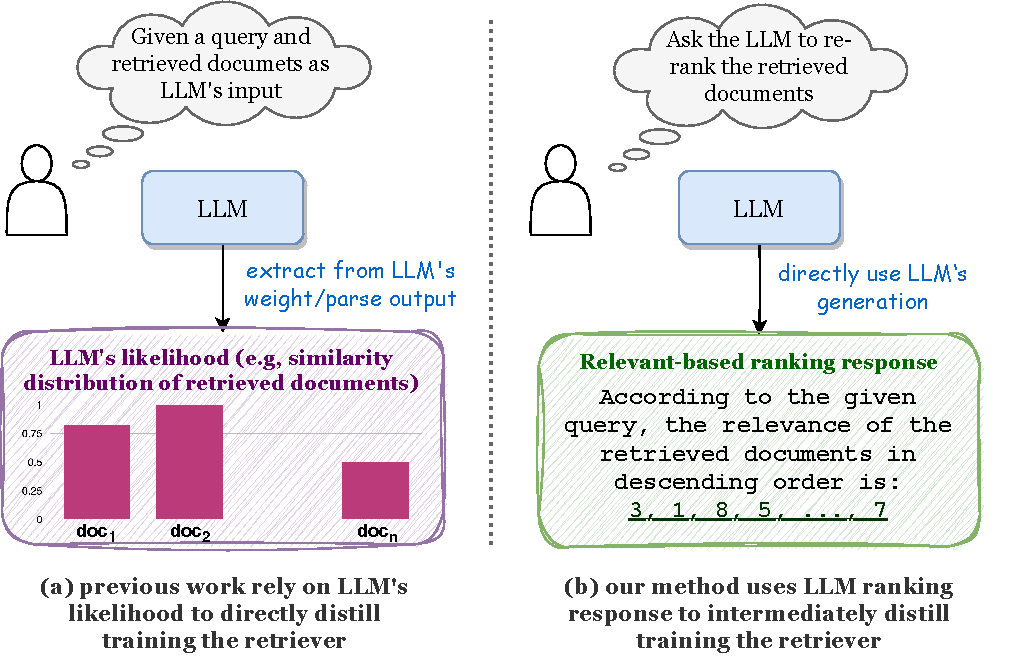
\includegraphics[width=0.5\textwidth]{latex/pic/fig1.pdf} % Reduce the figure size so that it is slightly narrower than the column.
    \caption{Previous distillation methods (left) rely on extracting supervision signals from LLM's weights or using LLM's output probabilities to train the retriever model. 
    In contrast, our approach (right) bypasses the need for LLM's likelihood, directly using the LLM's ranking responses as supervision signals.}
    \label{fig:01}
    \vspace{-5mm}  % 调整与下文的间距
\end{figure}


The retrieval-augmented generation (RAG) framework has been widely adopted to alleviate hallucination problems in LLMs generation, especially for knowledge-intensive tasks \cite{lewis2020retrieval}. 
The RAG framework consists of two key components: a retriever to locate relevant information from a large corpus based on a given input, and a reader, typically a LLM, to integrate this information into its generation \cite{izacard2023atlas, shi2023replug}. 

% to enhance the content generation.
% Influenced by such impressive performance, there are also numerous studies which have explored how to effectively leverage the capabilities of LLMs to complement information retrieval models, leading to the development of joint-training in Retrieval-augmented Generation (RAG) framework \cite{lewis2020retrieval}. 

% During the inference stage, the information retrieved by the retriever improves the accuracy of the reader’s output and reduces the frequency of hallucination responses.

% traditional retrieval algorithms and 
% Moreover, unlike using the retrieval algorithms or off-the-shelf models, jointly training RAG further enhances the performance of the retriever from another perspective. Specifically, it uses the powerful semantic alignment capabilities of LLMs to distill and train the retrieval model, thereby improving the overall performance of the RAG framework.

How to distill knowledge from LLMs to optimize the retriever in the RAG framework with in-domain data has been a crucial challenge. 
Early efforts proposed training the retriever with white-box LLM readers by extracting supervision signals directly from the LLMs' weights \cite{izacard2023atlas, rubin2023long, guu2020retrieval}. 
However, this approach becomes more computationally intensive and time-consuming as LLMs increase in size.
Meanwhile, it is incompatible with closed-source models.

Recently, researchers have also turned to knowledge distillation for the retriever from black-box LLMs by training the retriever directly from generated outputs, such as RePLUG \cite{shi2023replug} and In-Context RALM \cite{ram2023context}. 
However, both methods use the generation log probabilities for correct answers as the distillation signal to train the retriever, which may suffer from: 
1) Limited application scenarios, as the output probabilities are not always available for closed-source LLMs. 
2) Discrepancy between retrieval and generation, where training LLMs' next-token prediction is not optimal for retriever training.
3) High computing costs, since hundreds of thousands of training instances are required in their training process.

To address these limitations, we propose \textit{Intermediate Distillation}, a data-efficient training scheme that leverages LLM-generated ranking responses to guide the training of the retriever. 
Our model employs a rerank-then-retrieve pipeline, where LLMs indirectly influence the retriever training via an intermediate ranker model.
We chose this pipeline for three main reasons:
% Specifically, we first leverage the generated reranking responses to distill a smaller re-ranker model. Based on this, we further utilize this well-trained re-ranker model to distillation training a small retriever model, thereby intermediately transferring part of the retrieval capabilities of the large language model to the smaller retriever. 
% Instead of direct distilling the retriever model, we use a rerank-then-retriever pipeline to let LLM intermediately guide the training of retriever model, and the reasons are mainly twofold. 
1) The robust zero-shot ranking capabilities of LLMs establish a strong foundation for knowledge distillation.
2) Using LLMs to generate a relevance-based ranking order is more suitable for retriever training than depending on LLMs output probabilities, making the supervision signals more reliable.
3) There are no restrictions on accessing this generated ranking order.
% the re-ranking capability of LLMs for retrieved documents according to its relevance to the query prompt is more reliable than their direct ability to scale the relevance of retrieved documents. 
% Compared to the former, generating natural language responses is much more challenging for the latter to provide more accurate answers for large language models.
% Second, as previous research has found, the learning ability of the small-scale retrievers is limited. Introducing a re-ranker model with stronger data fitting ability as a learning intermediary helps them better assimilate the knowledge from large language models. 

Specifically, we first train a ranker model using the ranking orders generated by LLMs as supervision signals. We then employ this trained ranker to further train the retriever model.
We conduct a series of experiments using advanced, closed-source LLMs that restrict output probability access.
The empirical results demonstrate the effectiveness of our method, requiring 100x to even 1000x less data than previous methods \cite{ram2023context, shi2023replug}, thereby significantly reducing computational costs.
% Specifically, our training starts with an off-the-shelf retriever model that searches for relevant documents from a large corpus and then form a subset of relevance retrieved documents for a specific given query.
% We concatenate this query with all documents in this subset to create an input prompt for the LLM. 
% The LLM then generates a ranking list based on the relevance of the documents, which is used to unsupervised train a ranker model.
% This ranker model, initially starting with an off-the-shelf retriever checkpoint, is trained for the distillation training of the retriever model.
% Subsequently, this distilled ranker model provides unsupervised training signals to the retriever model, which also starts from an off-the-shelf retriever checkpoint. 
% This method effectively transfers the LLM's advanced semantic alignment capabilities to the smaller retriever model, enhancing its accuracy in identifying the relevant documents.
% Specifically, we initialize our training framework by using an off-the-shelf retriever model to search several documents from large corpus based on the given query, as the candidate document pool for ranking. 
% Then, we concatenate the query and all of the documents in the candidate pool to reform an input prompt for LLM, letting it generate a ranking list according to the <query, document> pair relevance, which could used for distill training a ranker model. 
% We further utilize this well-trained re-ranker model to unsupervised training the off-the-shelf retriever model mentioned above, thereby intermediately transferring the semantic alignment capability the LLMs have to the smaller retriever model. 
% We conduct a series of empirical experiments using various LLMs to demonstrate the effectiveness of our proposed distillation framework.
% We also compare our method with other supervised training signals, such as NLP task evaluation metrics, showcasing the superiority of our method. 
% Furthermore, we integrate our well-trained retriever models into the RAG framework and assess their performance in question-answering tasks.
% The experimental results further validate the universality and adaptability of our distillation approach.
Our main contributions are:
% \vspace{-20pt}
\begin{itemize}
    \setlength{\itemsep}{-2pt}
    \item We introduce Intermediate Distillation, a data-efficient knowledge distillation training scheme that optimizes retrieval models from black-box LLMs via an intermediate ranker model in a two-stage process.
    \item We conduct extensive experiments with cutting-edge LLMs and demonstrate the efficacy and efficiency of the proposed method in enhancing information retrieval performance compared to other supervision signals.
    \item We deploy our distilled retriever model within the RAG framework and demonstrate its effectiveness in downstream tasks such as open-domain question-answering.
   
\end{itemize}



% Meanwhile, the presence of the Retrieval-augmented Generation (RAG) framework \cite{lewis2020retrieval} has further enhanced the quality of LLMs' responses.
% That is, by leveraging the retriever model which dynamically searches the relevant information feed to the language model for generation, the corresponding responses become more accurate and the frequency of the hallucinations also reduces compared to using the vanilla language model.

% However, it has been a great challenge for the RAG framework to retrieve the passages that are most likely to be the target answers from a large amount of corpus, as training a high-quality retriever model is time-consuming and 

% Influenced by the large language models' impressive performance, previous works have explored the retrieve ability of LLM fine-tuning it as a retriever or a re-ranker, which shows the fine-tuned LLM achieves state-of-the-art performance, surpassing previous smaller retriever models. However, huge computational and time resources are needed to fine-tune a large language model before it becomes a high-quality retriever model. In this context, exploring how to utilize the capabilities of large language models more cost-effectively has become a valuable research question. 